\chapter{Evaluation}\label{evalChapter}

After explaining the two approaches, they are now compared on the tasks
outlined at the beginning (\Cref{introductionChapter}): how good are they at
predicting the tactical themes in a puzzle (\Cref{evalS1}), and how good are
they at predicting the difficulty of a puzzle (\Cref{evalS2})?

Each of the methods is evaluated in greater detail (\Cref{evalS3,evalS4}),
focusing on their individual advantages and disadvantages
(\Cref{evalS31,evalS41}).

Finally, each method has a unique application that the other does not: a game
review for the deep learning transformer approach (\Cref{evalS32}) and a
similarity comparison for the tree-based approach (\Cref{evalS42}). These are
discussed and judged based on their own merits.


\section{Prediction of Puzzle Themes}\label{evalS1}

Both approaches (\Cref{mlChapter,treeChapter}) are compared with the unseen
test set. The deep learning approach produced a model which can be tested
against the entire test set with no further modifications, while the $k$-NN
method (\Cref{treeS3}) is used to evaluate the tree-based approach. Due to its
computational complexity (\Cref{treeS31}), $k$-NN uses a subset of 100,000
puzzles of the training set and is evaluated against a random selection of
2,000 puzzles from the test set. This, of course, increases variance in the
final evaluation of the model, but is unavoidable without great investments in
time and processing power.

Per-label precision, recall, and F1-scores are considered for both approaches
(\Cref{labelTable}). Additionally, the averaged statistics are also shown. In
all averaging formats (micro, macro, weighted, sample), the deep learning
transformer model outperforms the tree-based $k$-NN approach, but it is
surprisingly close. 

The macro average (unweighted mean of the statistics) suffers greatly for both
approaches. This is due to the heavily unbalanced dataset
(\Cref{lichessDataExpl}), so the weighted average (more common themes have a
higher weight) is more appropriate.

The theme breakdown, despite being difficult to parse, shows some interesting
differences between the models' performances. All themes discussed in this
section are highlighted in \Cref{labelTable} for ease of readability. The
tree-based algorithm, which uses Stockfish for tree generation
(\Cref{treeS12}), is perfect at identifying \texttt{mateIn1} and almost perfect
at \texttt{mateIn2}. This is likely because mating patterns are quite common
and the meaningful move trees constructed for them are almost identical. For
this same reason, the tree-based model outperforms the deep learning
transformer model at \texttt{oneMove} and \texttt{short} label prediction.

On the other hand, the deep learning transformer model is almost completely
accurate at predicting \texttt{middlegame} and \texttt{endgame} labels, along
with the various types of endgame: \texttt{bishopEndgame},
\texttt{knightEndgame}, \texttt{pawnEndgame}, \texttt{queenEndgame},
\texttt{queenRookEndgame}, and \texttt{rookEndgame}. This is almost certainly a
result of the model being designed in a way where it can access the whole board
at once, and an absence of many pieces (which is a giveaway that a position is
in an endgame), is trivial for it to detect. 


\begin{table}[H]
  \centering
  \begin{adjustbox}{width=\textwidth}
    \begin{tabular}{l|rrrr|rrrr}
      & \multicolumn{4}{c}{Tree-Based $k$-NN} & \multicolumn{4}{c}{Deep Learning Transformer} \\
      Theme & Precision & Recall & F1-score & Support & Precision & Recall & F1-score & Support \\
      \hline

      advancedPawn&0.7660&0.3600&0.4898&100&0.7044&0.4462&0.5463&43215\\
      advantage&0.5693&0.4091&0.4761&572&0.5966&0.5898&0.5932&235529\\
      anastasiaMate&1.0000&0.3333&0.5000&3&0.8554&0.5338&0.6574&798\\
      arabianMate&0.0000&0.0000&0.0000&1&0.7858&0.5842&0.6702&760\\
      attackingF2F7&0.8333&0.5556&0.6667&9&0.8693&0.7412&0.8002&4657\\
      attraction&0.9697&0.4156&0.5818&77&0.6858&0.1767&0.2810&26566\\
      backRankMate&0.6607&0.5692&0.6116&65&0.8236&0.8427&0.8330&24332\\
      \rowcolor{lightgray} bishopEndgame&0.7778&0.4667&0.5833&15&0.9622&0.9774&0.9697&9476\\
      bodenMate&0.0000&0.0000&0.0000&2&0.8045&0.5619&0.6617&315\\
      capturingDefender&0.0000&0.0000&0.0000&13&0.7120&0.0209&0.0406&6505\\
      castling&0.0000&0.0000&0.0000&2&0.5000&0.0071&0.0141&421\\
      clearance&0.5000&0.0400&0.0741&25&0.7768&0.0320&0.0616&10641\\
      crushing&0.7094&0.6704&0.6893&892&0.7223&0.5972&0.6538&337162\\
      defensiveMove&0.5000&0.1121&0.1832&107&0.5340&0.0462&0.0850&47212\\
      deflection&0.7857&0.1341&0.2292&82&0.7243&0.0940&0.1664&32867\\
      discoveredAttack&0.7778&0.2823&0.4142&124&0.6760&0.2641&0.3799&43352\\
      doubleBishopMate&0.0000&0.0000&0.0000&0&0.7907&0.5795&0.6689&352\\
      doubleCheck&0.0000&0.0000&0.0000&8&0.7518&0.2327&0.3554&3670\\
      dovetailMate&0.0000&0.0000&0.0000&2&0.7222&0.0323&0.0619&402\\
      enPassant&0.0000&0.0000&0.0000&0&0.7333&0.0189&0.0368&1165\\
      \rowcolor{lightgray} endgame&0.8036&0.7412&0.7711&966&0.9984&0.9999&0.9992&368846\\
      equality&0.0000&0.0000&0.0000&23&1.0000&0.0001&0.0002&8503\\
      exposedKing&0.0000&0.0000&0.0000&54&0.3561&0.1114&0.1697&21239\\
      fork&0.7500&0.5445&0.6309&281&0.7666&0.4015&0.5270&111331\\
      hangingPiece&0.6538&0.2073&0.3148&82&0.6806&0.1650&0.2657&33331\\
      hookMate&0.0000&0.0000&0.0000&5&0.6887&0.4616&0.5527&1107\\
      interference&0.0000&0.0000&0.0000&9&0.6250&0.0016&0.0032&3129\\
      intermezzo&1.0000&0.0357&0.0690&28&0.7517&0.0402&0.0763&11221\\
      kingsideAttack&0.7742&0.3357&0.4683&143&0.7146&0.6082&0.6571&61522\\
      \rowcolor{lightgray} knightEndgame&0.7000&0.4667&0.5600&15&0.9319&0.9944&0.9621&5887\\
      long&0.6809&0.1932&0.3009&497&0.5746&0.0754&0.1333&193731\\
      master&0.0000&0.0000&0.0000&148&0.2500&0.0001&0.0001&54003\\
      masterVsMaster&0.0000&0.0000&0.0000&11&0.0000&0.0000&0.0000&4967\\
      mate&0.9783&0.9688&0.9735&512&0.8210&0.7731&0.7963&198507\\
      \rowcolor{lightgray} mateIn1&1.0000&1.0000&1.0000&219&0.7483&0.6803&0.7127&80324\\
      \rowcolor{lightgray} mateIn2&0.9773&1.0000&0.9885&215&0.7727&0.5100&0.6145&91787\\
      mateIn3&0.9388&0.6866&0.7931&67&0.7096&0.2987&0.4204&22611\\
      mateIn4&0.6667&0.2500&0.3636&8&0.5562&0.0322&0.0608&3076\\
      mateIn5&0.0000&0.0000&0.0000&3&0.9062&0.0409&0.0783&709\\
      \rowcolor{lightgray} middlegame&0.7285&0.7293&0.7289&931&0.9919&0.9854&0.9886&377218\\
      \rowcolor{lightgray} oneMove&1.0000&0.8939&0.9440&245&0.7566&0.6041&0.6718&89681\\
      opening&0.5909&0.1262&0.2080&103&0.8873&0.9419&0.9138&44379\\
      \rowcolor{lightgray} pawnEndgame&0.7846&0.9623&0.8644&53&0.9742&0.9998&0.9868&22943\\
      pin&0.8261&0.1397&0.2390&136&0.6821&0.2167&0.3288&49568\\
      promotion&1.0000&0.0968&0.1765&31&0.6591&0.3415&0.4499&16317\\
      \rowcolor{lightgray} queenEndgame&1.0000&0.2500&0.4000&16&0.9748&0.9915&0.9830&7282\\
      \rowcolor{lightgray} queenRookEndgame&0.0000&0.0000&0.0000&17&0.9482&0.9170&0.9324&5171\\
      queensideAttack&0.7143&0.1471&0.2439&34&0.5973&0.4695&0.5257&10552\\
      quietMove&0.9231&0.1579&0.2697&76&0.5908&0.1497&0.2388&31019\\
      \rowcolor{lightgray} rookEndgame&0.7400&0.3814&0.5034&97&0.9759&0.9893&0.9826&37058\\
      sacrifice&0.8571&0.3947&0.5405&152&0.7042&0.2853&0.4061&55181\\
      \rowcolor{lightgray} short&0.7341&0.8385&0.7829&1090&0.6810&0.6802&0.6806&434161\\
      skewer&0.6667&0.2927&0.4068&41&0.7135&0.2891&0.4115&17291\\
      smotheredMate&0.5000&0.2500&0.3333&4&0.8920&0.8392&0.8648&2264\\
      superGM&0.0000&0.0000&0.0000&0&0.0000&0.0000&0.0000&462\\
      trappedPiece&1.0000&0.1481&0.2581&27&0.6613&0.1431&0.2352&11135\\
      underPromotion&0.0000&0.0000&0.0000&0&0.0000&0.0000&0.0000&140\\
      veryLong&0.7500&0.0180&0.0351&167&0.6098&0.0084&0.0166&62128\\
      xRayAttack&0.0000&0.0000&0.0000&5&0.7980&0.2401&0.3691&2699\\
      zugzwang&0.4444&0.2000&0.2759&20&0.7079&0.3097&0.4308&6604\\
      \hline
      micro~avg&0.7774&0.5869&0.6689&8630&\textbf{0.8025}&\textbf{0.6040}&\textbf{0.6893}&3388481\\
      macro~avg&0.5339&0.2801&0.3324&8630&\textbf{0.7065}&\textbf{0.3996}&\textbf{0.4497}&3388481\\
      weighted~avg&0.7416&0.5869&0.6211&8630&\textbf{0.7600}&\textbf{0.6040}&\textbf{0.6388}&3388481\\
      samples~avg&0.7501&0.5952&0.6488&8630&\textbf{0.8063}&\textbf{0.6181}&\textbf{0.6734}&3388481\\
    \end{tabular}
  \end{adjustbox}
  \caption{Label breakdown of precision, recall, and F1-score for the two models.}
  \label{labelTable}
\end{table}


\section{Prediction of Puzzle Difficulty}\label{evalS2}

Both methods were also evaluated on their ability to correctly predict
difficulty rating of puzzles. To measure their performance, the average root
mean squared error and $r^2$ score was calculated over the entire test set
(\Cref{diffTable}). As before, the tree-based $k$-NN method was only tested on
2,000 samples due to its slow inference time. 

A random sample of 1,000 puzzles, along with their actual and predicted
difficulty ratings, are also shown for each method
(\Cref{predTree,predTransformer}).

From the results, we see that the tree-based $k$-NN is considerably better than
the transformer-based model at predicting difficulty rating, with a root mean
square error of 64 points lower. Additionally, its $r^2$-score is much higher.
It should be noted that this model was evaluated on far fewer samples, but
despite this, its performance is very good.

It is interesting that the transformer-based model tends to overshoot the
rating when it is low, and tends to predict a lower rating when it is high
(\Cref{errTransformer}). This is likely a result of slight overfitting, or a
consequence of the loss function used.

\begin{table}[H]
  \centering
  \begin{tabular}{l|rr}
    Metric & Tree-Based $k$-NN & Deep Learning Transformer \\
    \hline
    $r^2$ score & \textbf{0.4256} & 0.2593 \\
    Root mean squared error & \textbf{404.5} & 468.4 \\
  \end{tabular}
  \caption{Metrics of success for difficulty prediction.}
  \label{diffTable}
\end{table}

\begin{figure}[H]
  \begin{minipage}{0.475\textwidth}
    \centering
    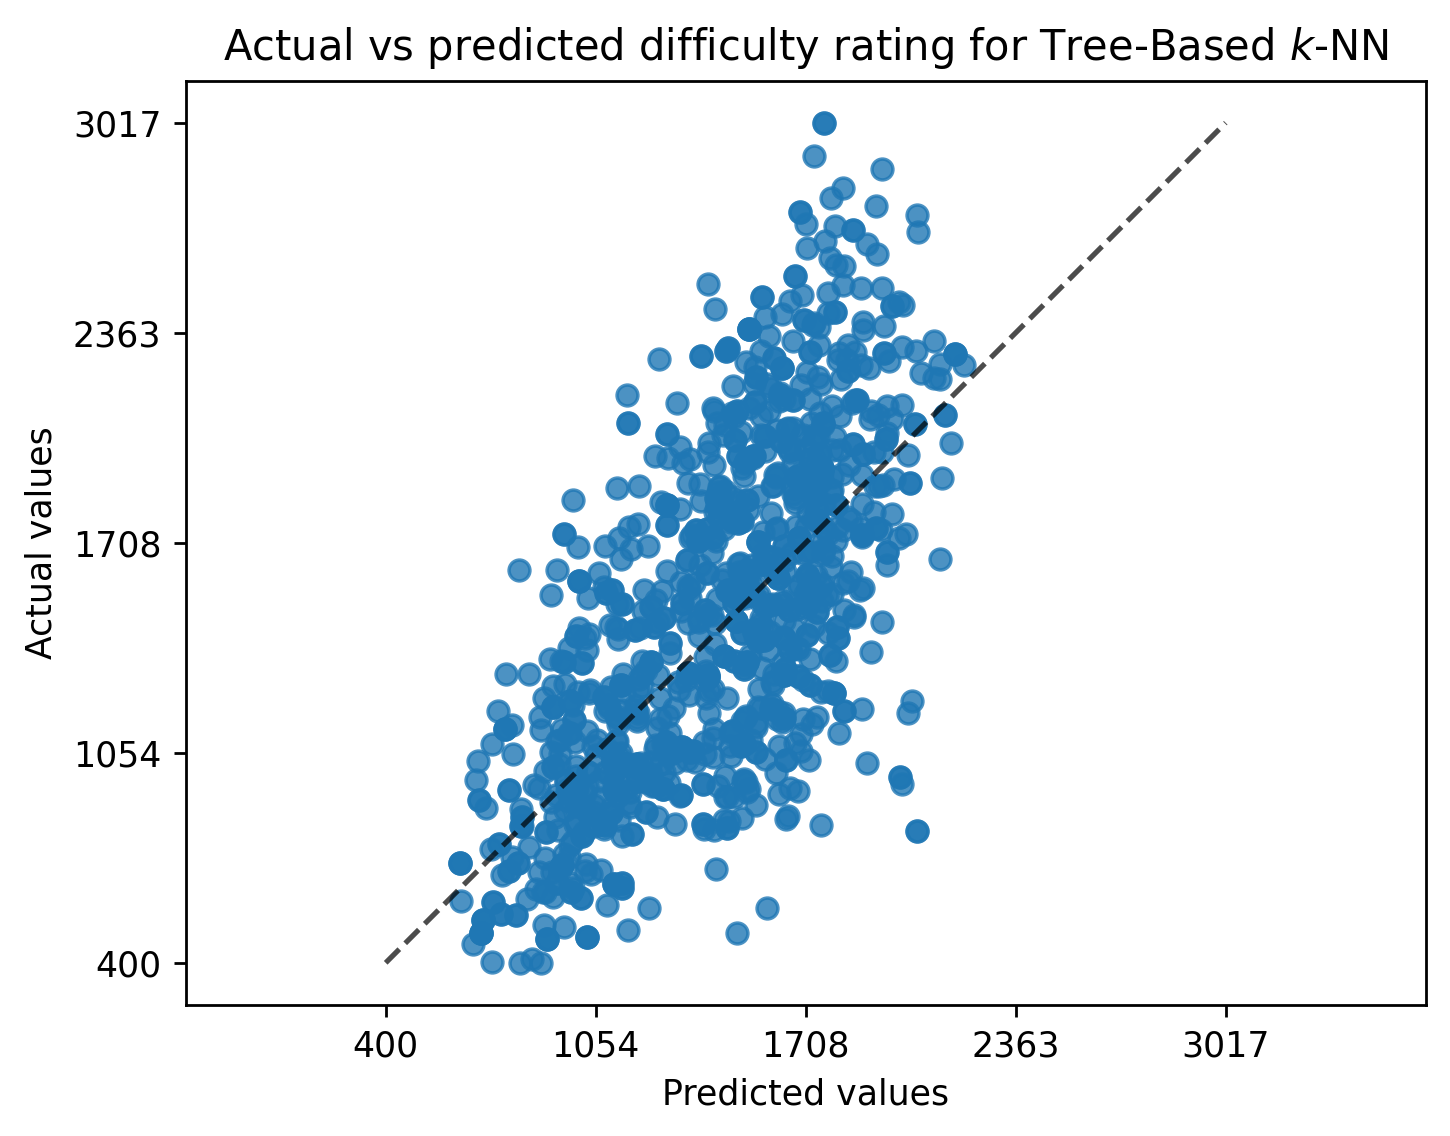
\includegraphics[width=\textwidth]{evaluation/img/tree.png}
    \caption{Actual vs predicted ratings for the tree-based $k$-NN method.}
    \label{predTree}
  \end{minipage}
  \hspace{0.05\textwidth}
  \begin{minipage}{0.475\textwidth}
    \centering
    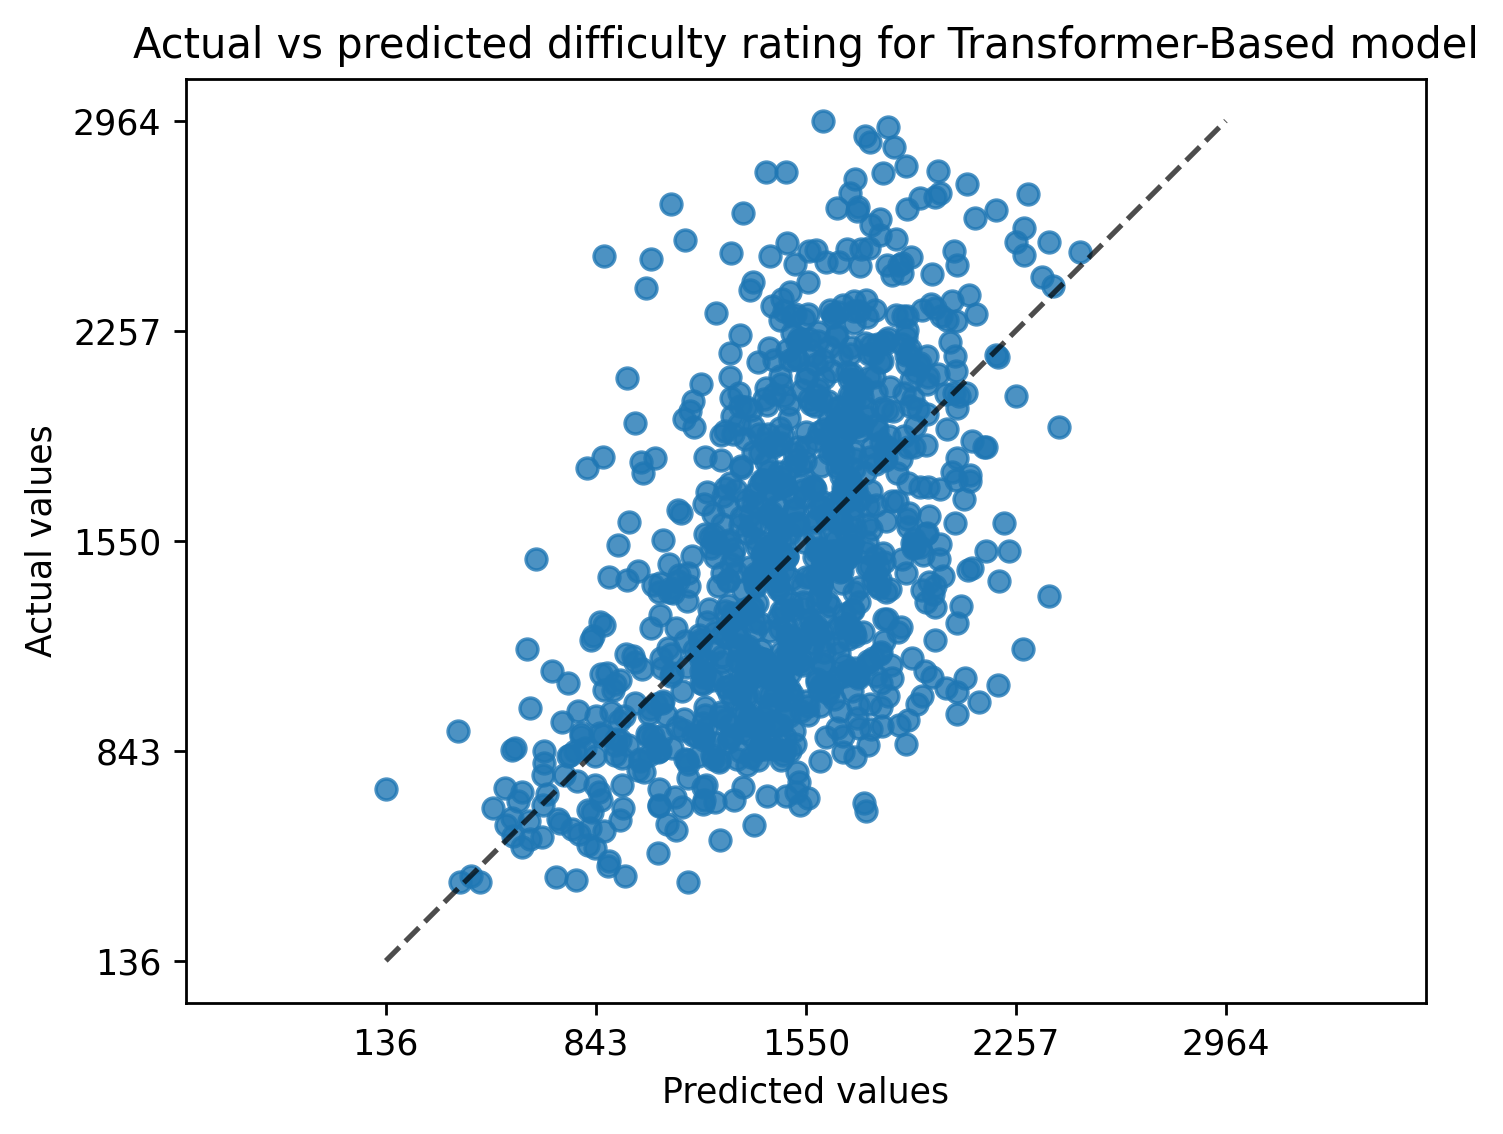
\includegraphics[width=\textwidth]{evaluation/img/transformer.png}
    \caption{Actual vs predicted ratings for the transformer-based model.}
    \label{predTransformer}
  \end{minipage}
\end{figure}

\begin{figure}[H]
  \begin{minipage}{0.475\textwidth}
    \centering
    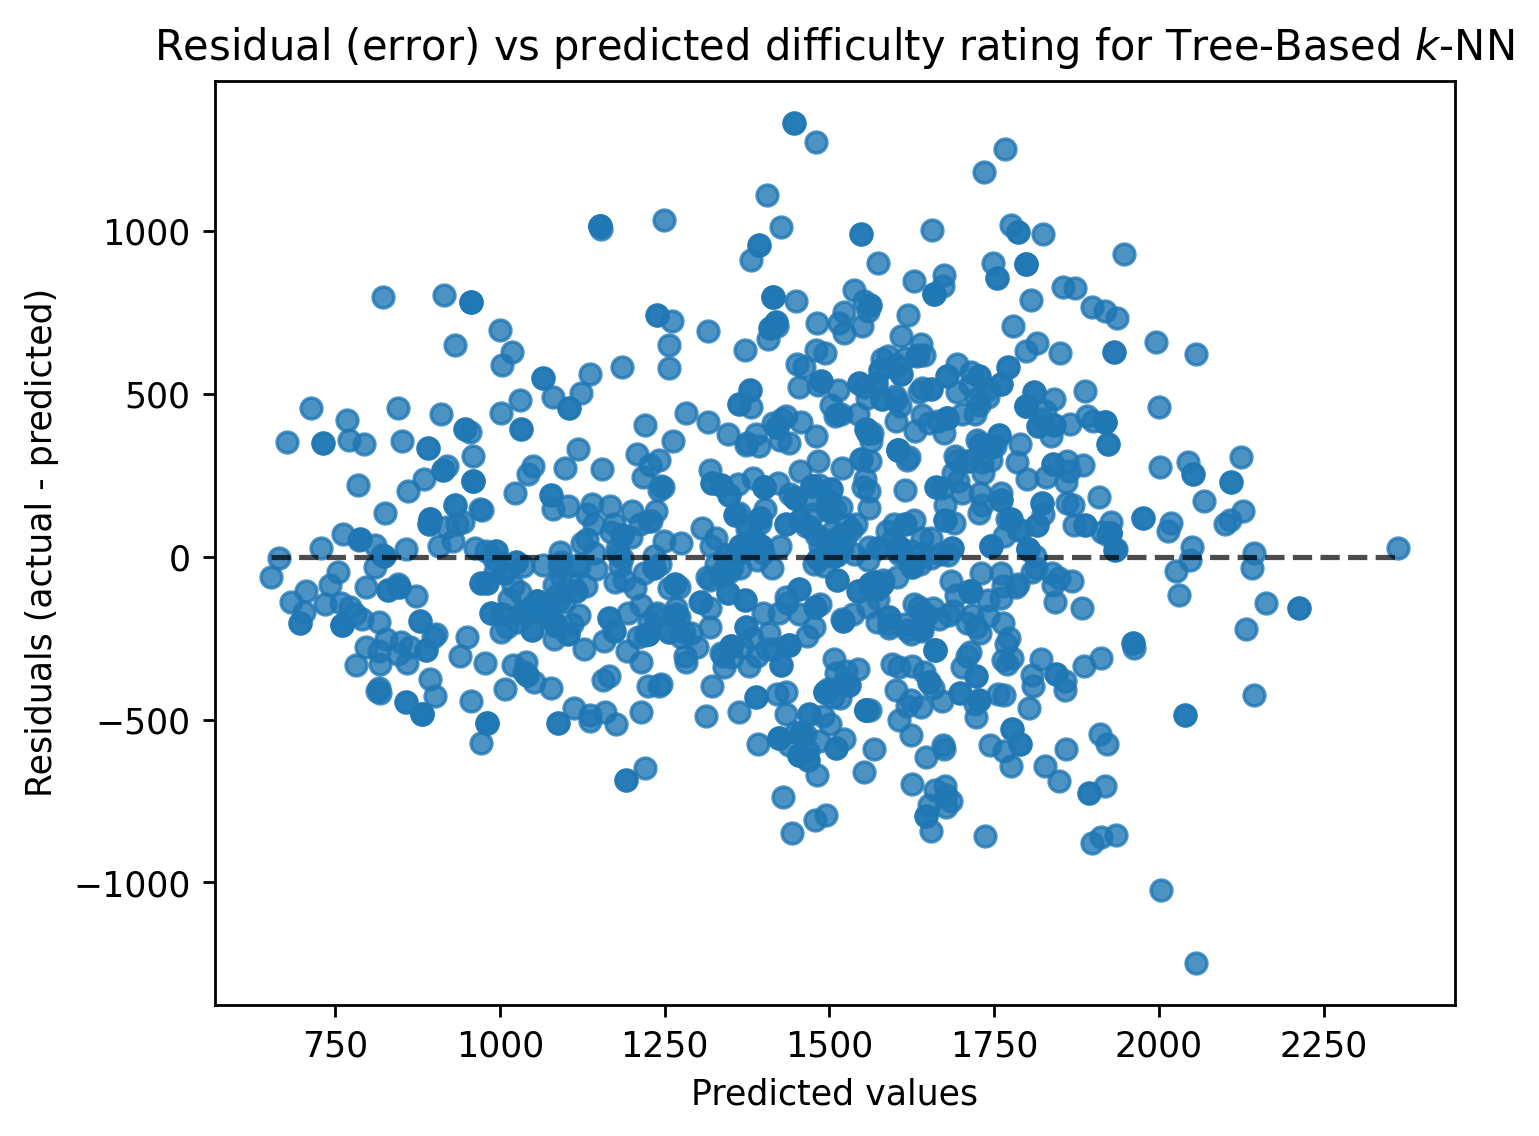
\includegraphics[width=\textwidth]{evaluation/img/tree_err.png}
    \caption{Residuals vs predicted ratings for the tree-based $k$-NN method.}
    \label{errTree}
  \end{minipage}
  \hspace{0.05\textwidth}
  \begin{minipage}{0.475\textwidth}
    \centering
    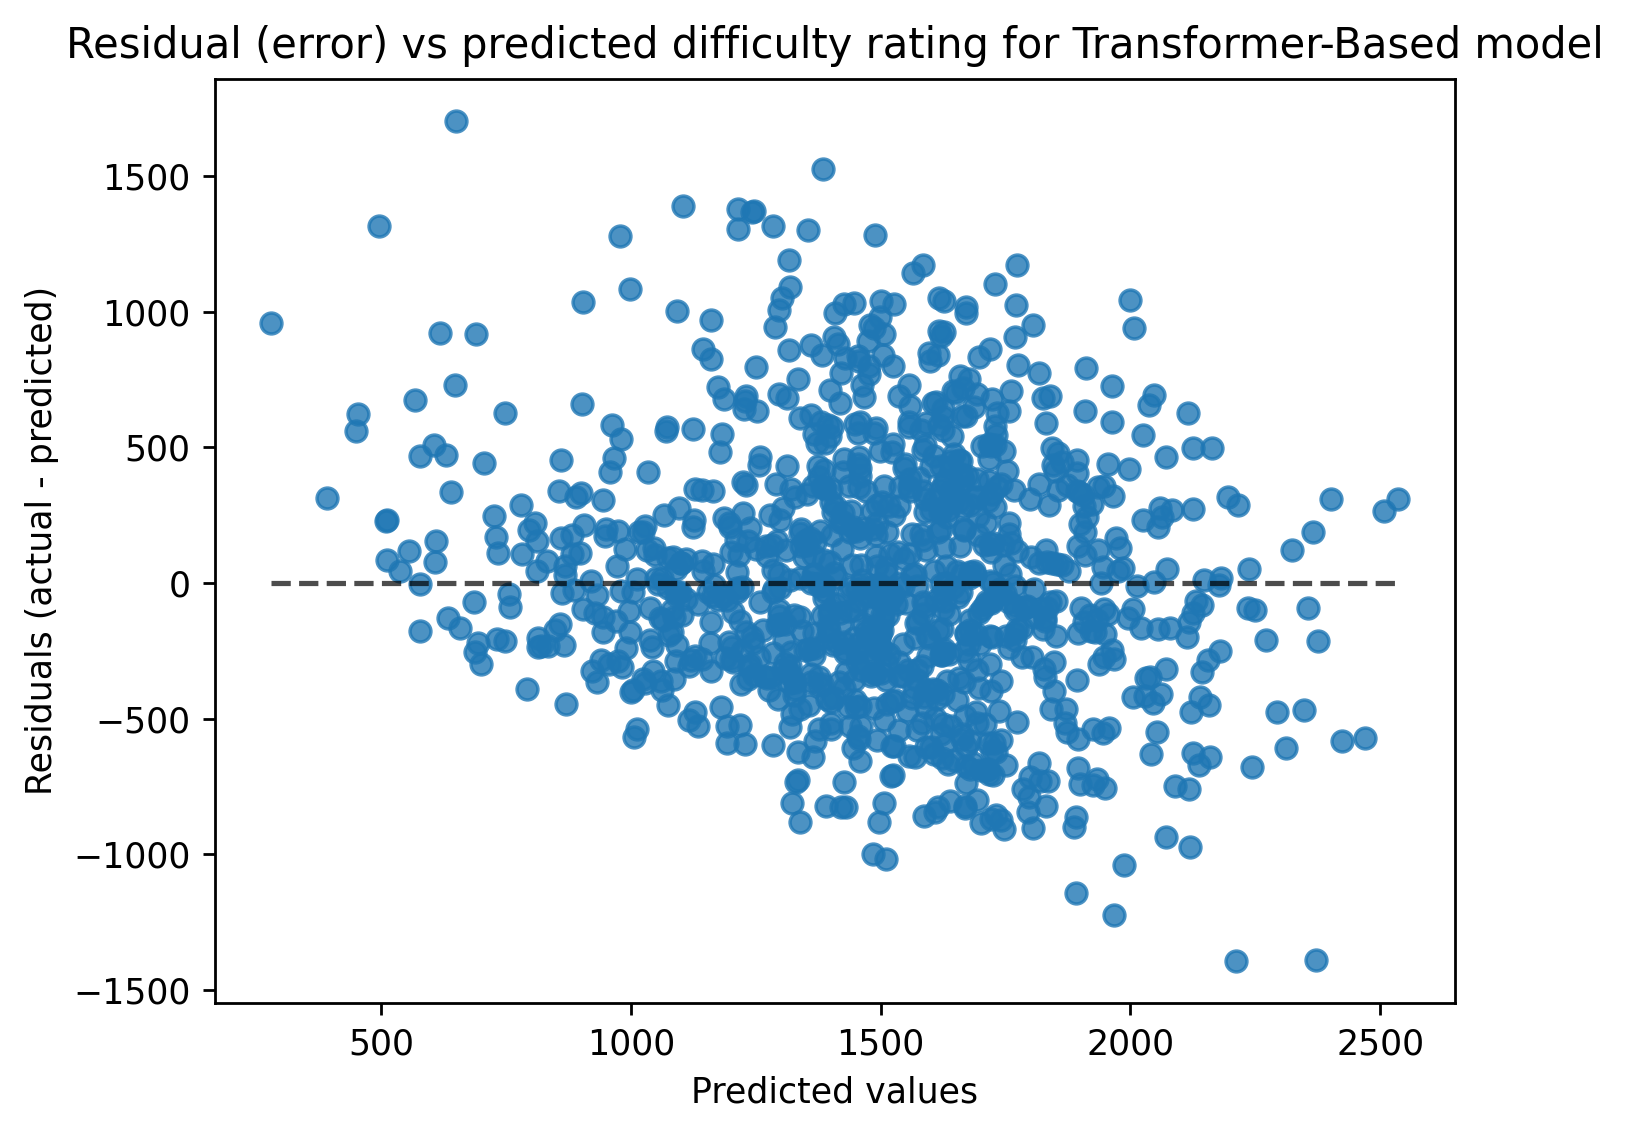
\includegraphics[width=\textwidth]{evaluation/img/transformer_err.png}
    \caption{Residuals vs predicted ratings for the transformer-based model.}
    \label{errTransformer}
  \end{minipage}
\end{figure}


\section{Deep Learning Approach}\label{evalS3}

\subsection{Strengths and Weaknesses}\label{evalS31}

The advantages of this approach are clearly the better performance
(\Cref{labelTable}) compared to the tree-based approach. After a relatively
long training period, the models produced by this method can analyse new
positions almost instantly. As the output of the model is a number in the range
$(0, 1)$, a sense of `confidence' in the output can also be easily understood,
which is considerably more difficult in the tree-based approach with $k$-NN.

The biggest downside is the trade-off of having fast inference: slow training
time. This, combined with the need to search for hyperparameters (\Cref{mlS22})
makes this method quite time and resource intensive. The deep learning method
also requires a lot of access to chess puzzle data, which can be of varying
quality. This also means that it cannot learn new puzzle tactic patterns if
they are not labelled appropriately.

\subsection{Game Review}\label{evalS32}

An interesting unintended feature of this approach is that it can, of course,
predict puzzle themes for any chess position. Since inference time is so fast,
it is possible to iterate through any chess game's moves and analyse those
positions. For this example, a game played by the authors was analysed, and the
interesting positions, along with their labels, are shown below. Interestingly,
the starting position (\Cref{alapin1}) has the labels \texttt{crushing},
\texttt{hangingPiece}, and \texttt{oneMove}. The model does correctly predict
\texttt{opening}. 

After playing a strange sequence of pawn moves (\Cref{alapin2}), Black gets a
losing position, where White has a classic \emph{attack on f7} tactic. Indeed,
White's best move in this position is a \emph{bishop sacrifice},
\texttt{9.Bxf7+ Kxf7}, which walks into a knight check: \texttt{10.Ng5+ Ke8
11.Qxg4}. Right before the \emph{bishop sacrifice} was played, the model
correctly predicts \texttt{attackingF2F7}, \texttt{attraction} (the black king
is attracted onto a square where it can be checked by the knight) and
\texttt{sacrifice}. These themes appear only at this position, and nowhere else
in the game. As a side note, the position immediately prior to \texttt{10.Ng5+}
is labelled \texttt{discoveredAttack}. It is also at this point that the model
stops predicting \texttt{opening} and begins predicting \texttt{middlegame}.

This attack leads to what seems to be a mating position (\Cref{alapin3}).
Despite this, White does not have a checkmate. The player with the white pieces
testifies that he thought the position must have a forced mate, and the model
agrees, predicting \texttt{mate} and \texttt{mateIn1}. Both are wrong.

After many moves, White fails to convert his advantage (\Cref{alapin4}), and
ends up in an equal position. After the rook trade, \texttt{30...Rxe1+ 31.Rxe1
Bxd4}, the model switches its predictions from \texttt{middlegame} to
\texttt{endgame}. No more sharp positions appear for the rest of the game and
the model's predictions are equally uninteresting.

\begin{figure}[H]
  \begin{minipage}[t]{0.475\textwidth}
    \centering
    \chessboard[setfen=rnbqkbnr/pppppppp/8/8/8/8/PPPPPPPP/RNBQKBNR w KQkq - 0 1]
    \caption{The starting position.}
    \label{alapin1}
  \end{minipage}
  \hspace{0.05\textwidth}
  \begin{minipage}[t]{0.475\textwidth}
    \centering
    \chessboard[setfen=2rqkbnr/3npppp/p2p4/1ppB4/3PP1b1/2P2N2/PP3PPP/RNBQ1RK1 w k - 0 9]
    \caption{White has a winning advantage.}
    \label{alapin2}
  \end{minipage}
\end{figure}

\begin{figure}[H]
  \begin{minipage}[t]{0.475\textwidth}
    \centering
    \chessboard[setfen=2rqkb1r/4p1pp/pn1pQn2/1pp3N1/3PP3/2P5/PP3PPP/RNB2RK1 w - - 3 13]
    \caption{Despite looking lethal for Black, White does not have a forced mate.}
    \label{alapin3}
  \end{minipage}
  \hspace{0.05\textwidth}
  \begin{minipage}[t]{0.475\textwidth}
    \centering
    \chessboard[setfen=1r6/3kr1b1/3p3p/3n2p1/1p1P4/6N1/P2B1PPP/1R2R1K1 b - - 4 30]
    \caption{After the rook trade, White loses the \texttt{d4} pawn and loses the game soon after.}
    \label{alapin4}
  \end{minipage}
\end{figure}


\section{Tree-Based Approach}\label{evalS4}

\subsection{Strengths and Weaknesses}\label{evalS41}

The biggest weakness of the tree-based approach -- using $k$-NN to predict
labels and difficulty -- is the inference time. This has had large consequences
previously in the project, and this is an unavoidable result of using a
relatively expensive and non-vectorisable distance function. This downside
meant that the method could not be evaluated fully, as it was time prohibitive
to analyse the entire test set while using the entire training set.

Another downside is the sensitivity to parameters (\Cref{treeS13}). Different
parameters in the distance function define what it means for a puzzle to be
similar, and this, of course, can also vary drastically between chess players.
The other set of parameters that greatly influences the performance is the tree
generation parameters (\Cref{treeS12}). These are again non-trivial to
optimise, as it takes a long time to regenerate the meaningful search trees.
These parameters also change from person to person, especially the arbitrary
move consideration boundary, which was kept at 100 centipawns in this project.
It is very likely that a higher skilled player would not even consider
low-performing moves when comparing if two puzzles are similar, whereas a lower
rated player would calculate more variations deeper as he is unable to
understand the strength of a position with intuition alone.

However, within this weakness also lies the main strength of this method. This
tunability means chess players of all skills can benefit from the distance
function, as they can tweak it to their performance.

Of course, this also means this method of puzzle comparison is much more
explainable than the black-box deep learning approach. It is completely
possible to view a puzzle's meaningful move tree, and to reason about why a
certain puzzle is said to be close to another, or said to have a certain label
or difficulty.

\subsection{Puzzle Similarity}\label{evalS42}

Grouping puzzles (\Cref{treeS2}) and ranking puzzles by similarity
(\Cref{treeS21}) is unique to this method. Qualitative analysis of clustering
performance has been shown to have intriguing results (\Cref{treeS23}), as this
method was able to group together puzzles in ways that have not been
implemented before. The distance-based method of ranking puzzles by similarity
is also promising, and can likely be used to datamine game databases to find
similar positions. 

